\documentclass{standalone}
\usepackage{pgfplots}
\pgfplotsset{compat=1.18}
\usetikzlibrary{arrows.meta}

\begin{document}

\definecolor{tab_blue}{HTML}{1F77B4}
\definecolor{tab_orange}{HTML}{FF7F0E}
\definecolor{tab_green}{HTML}{2CA02C}
\definecolor{tab_red}{HTML}{D62728}

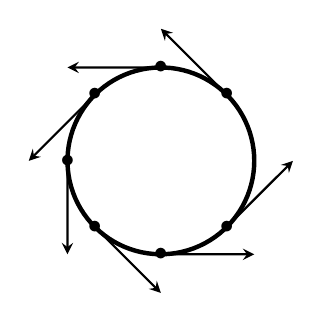
\begin{tikzpicture}
\begin{axis}[
% axis on top,
% axis lines = box,
axis lines = none,
unit vector ratio=1 1, 
% axis equal=false,
scale=1.0, 
xmin=-1.6, xmax=2.6, ymin=-2.0, ymax=2.8, 
grid = major,
declare function={ 
    myfunc(\x) = 0.5*\x+0.3*sin(deg(pi*\x));
    myfuncderiv(\x) = 0.5 + 0.3*pi*cos(deg(pi*\x)); 
    vecx(\x) = -\x; 
    vecy(\x) = \x;
}
]

\pgfmathsetmacro{\a}{0.0}
\pgfmathsetmacro{\b}{2.0*pi}
\pgfmathtruncatemacro{\Nsub}{8}
\pgfmathsetmacro{\h}{(\b-\a)/\Nsub}

\addplot[domain=\a:\b, samples=100, ultra thick] ({cos(deg(x))}, {sin(deg(x))});

\pgfplotsforeachungrouped \i in {1,...,\Nsub-1}{
    \pgfmathsetmacro{\xcoord}{cos(deg(\i*\h))} 
    \pgfmathsetmacro{\ycoord}{sin(deg(\i*\h))} 
    \pgfmathsetmacro{\temp}{vecx(\xcoord)*(-\ycoord) + vecy(\xcoord)*\xcoord}
    \edef\doplot{\noexpand 
        \node at (\xcoord,\ycoord) {$\bullet$};
    }
    \doplot
    \edef\doplot{\noexpand 
        \draw[->, >=stealth, thick] (\xcoord,\ycoord) -- ({\xcoord-\ycoord}, {\ycoord+\xcoord});
    }
    \doplot
}
% \draw[->, >=stealth, thick] (0,0) -- (1,1);
% \node at (0, 1) {$\bullet$}; 
% \pgfmathsetmacro{\pk}{cosh(1.0)}
% \node at (1.0, \pk) {$\bullet$}; 
% \addplot[domain=0:1, samples=100, ultra thick, color=tab_red] {cosh(x)}; 

\end{axis}
\end{tikzpicture}

\end{document}